\documentclass[../differential_geometry.tex]{subfiles}
\begin{document}
\section{Aula 05 - de Fevereiro, 2026}
\subsection{Motivações}
\begin{itemize}
	\item Contato com Círculos;
	\item Evoluta;
	\item Envelope das Retas Normais.
\end{itemize}
\subsection{Evoluta: definição e propriedades}
Veremos como funciona o contato de curvas com círculos, começando por deixar claro o que consideramos um círculo:
\begin{def*}
	O \textbf{círculo de centro c e raio r} é o conjunto dos pontos \(x=(x, y)\) do plano tal que
	\[
		\Vert x-c \Vert=r \Longleftrightarrow \langle x-c, x-c \rangle-r^{2}=0.\; \square
	\]
\end{def*}

O fenômeno que desejamos representar é o representado na imagem a seguir:
\begin{figure}[H]
	\begin{center}
		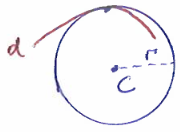
\includegraphics[height=0.4\textheight, width=0.4\textwidth, keepaspectratio]{./Images/contact_circle_05.png}
	\end{center}
\end{figure}

Para tanto, vamos considerar a função \(f(x, y)=\langle x-c, x-c \rangle-r^{2}\); o contato entre a curva \(\alpha \) e o círculo \(C(c, r)\) no ponto \(\alpha (s_{0})\) é medido pela função
\[
	g(s)=f(\alpha (s)) = \langle \alpha (s)-c, \alpha (s)-c \rangle-r^{2},
\]
e temos \(g(s_{0})=0\) se, e somente se, o valor de r é \(r=\Vert \alpha (s_{0})-c \Vert\), ou seja, quando \(\alpha (s_{0})\in C(c, r)\).

Suponha que \(g(s_{0})=0\), e tome \(\alpha \) parametrizada p.c.a; então, com respeito às derivadas, de g,
\begin{align*}
	 & \frac{1}{2}g'(s)=\langle t(s), \alpha (s)-c \rangle                                                               \\
	 & \frac{1}{2}g''(s) = \kappa (s)\langle n(s), \alpha (s)-c \rangle+1                                                \\
	 & \frac{1}{2}g'''(s)=\kappa '(s)\langle n(s), \alpha (s)-c \rangle-\kappa^{2}(s)\langle t(s), \alpha (s)-c \rangle,
\end{align*}
donde segue que
\begin{align*}
	g'(s) = 0 & \Longleftrightarrow [\alpha (s_{0})-c]\parallel n(s_{0})                             \\
	          & \Longleftrightarrow \alpha (s_{0})-c = \lambda n(s_{0}),\quad \lambda \in \mathbb{R} \\
	          & \Longleftrightarrow c=\alpha (s_{0})-\lambda n(s_{0}).
\end{align*}
Logo, todos os círculos que passam por \(\alpha (s_{0})\) e cujos centros pertencem à reta normal à curva \(\alpha \) em \(\alpha (s_{0})\) têm contato de ordem maior ou igual a 2 com a curva!

E quanto aos pontos de ordem maior ou igual que 3? Bom, fazendo um raciocínio semelhante ao feito para ordem maior ou igual a 2, vamos analisar quando que a derivada até segunda se anula:
\begin{align*}
	g(s_{0})=g'(s_{0})=g''(s_{0})=0 & \Longleftrightarrow \kappa (s_{0})\langle n(s_{0}), \lambda n(s_{0}) \rangle +1=0                                  \\
	                                & \Longleftrightarrow \lambda \kappa (s_{0})+1=0                                                                     \\
	                                & \stackrel{\mathclap{\text{Se }\kappa (s_{0})\neq 0}}\Longleftrightarrow \quad \lambda = - \frac{1}{\kappa (s_{0})} \\
	                                & \Longleftrightarrow  c = \alpha (s_{0})+\frac{1}{\kappa (s_{0})}n(s_{0}).
\end{align*}
Consequentemente, se o ponto \(\alpha (s_{0})\) \textbf{não é ponto de inflexão da curva}, então existe um círculo único que tem contato de ordem maior ou igual a 3 com \(\alpha \) em \(\alpha (s_{0}).\)
\begin{def*}
	Se \(\alpha (s_{0})\) não é ponto de inflexão da curva \(\alpha \), então o círculo descrito acima, ou seja, o único que tem contato de ordem maior ou igual que 3 com \(\alpha \) em \(\alpha (s_{0})\), é chamado \textbf{círculo osculador da curva}\footnote{Do latim \textit{oscular}, que significa basicamente beijar, então é ``o círculo que dá um selinho na curva''!} \(\alpha \) em \(\alpha (s_{0}).\; \square\)
\end{def*}

Uma propriedade muito interessante dos círculos osculadores é que o raio deles é exatamente \(1/\kappa (s_{0})\), ou seja, ganhamos outra definição da curvatura de uma curva plana: a curvatura de \(\alpha \) é o inverso do raio do círculo que tem contato maior ou igua a 3 com ela.

Variando \(s_{0}\) em I, podemos nos basear no raciocínio acima e obter uma outra curva plana parametrizada por \(e:I\rightarrow \mathbb{R}^{2}\) dada por
\[
	e(s)=\alpha (s)+\frac{1}{\kappa (s)}n(s).
\]
\begin{def*}
	A curva e é chamada \textbf{evoluta da curva \(\mathbf{\alpha }\)}. \(\square\)
\end{def*}

No quesito propriedades, de cara já sabemos que a evoluta é suave, pois \(\alpha, \; \kappa \) e \(n\) são todos suaves, até porque estamos assumindo que \(\kappa (s)\neq 0\) para todo ponto s.
Derivando ela, obtemos
\[
	e'(s)=t(s)+\frac{1}{\kappa (s)}(-\kappa (s)t(s))-\frac{\kappa '(s)}{\kappa^{2}(s)}n(s),
\]
ou seja,
\[
	\boxed{e'(s)=-\frac{\kappa'(s)}{\kappa^{2}(s)}n(s)},
\]
e obtemos a propriedade de que
\begin{quote}
	``A evoluta é regular num ponto da curva se, e somente se, este ponto não é um vértice da curva.''.
\end{quote}
Posto de outra forma, \textbf{as singularidades da evoluta detectam os vértices da curva!} Mais do que isso, se \(\alpha (s_{0})\) não é um vértice, a reta tangente à evoluta no ponto \(\alpha (s_{0})\) é a reta normal à curva \(\alpha \) no ponto \(\alpha (s_{0})\):
\begin{figure}[H]
	\begin{center}
		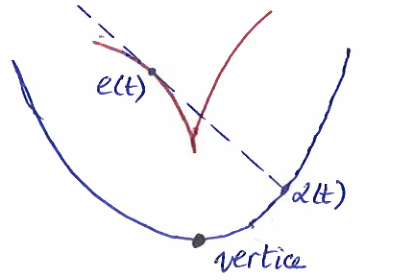
\includegraphics[height=0.6\textheight, width=0.6\textwidth, keepaspectratio]{./Images/evoluta_parabola_05.png}
	\end{center}
\end{figure}

\begin{exr}
	Encontre uma parametrização da evoluta da elipse parametrizada por \(\alpha (u)=(\alpha \cos^{}{u}, \alpha \sin^{}{u})\), com \(u\in \mathbb{R}\) e \(0<b<a\)
\end{exr}

\subsection{Envelope das Retas Normais}
Apesar de termos ganhado uma segunda caracterização da curvatura por meio da evoluta, ainda temos que fazer muita coisa para identificar seu valor ou expressão, além de todas as verificações necessárias.
Nosso próximo passo é justamente resolver parte deste problema: relacionaremos as evolutas à família dos \textit{envelopes das retas normais}, mas primeiro temos que entender o que é isso.

Considere a família de círculos unitários \((x-t)^{2}+y^{2}=1\), todos centrados em \((t, 0)\).
\begin{figure}[H]
	\begin{center}
		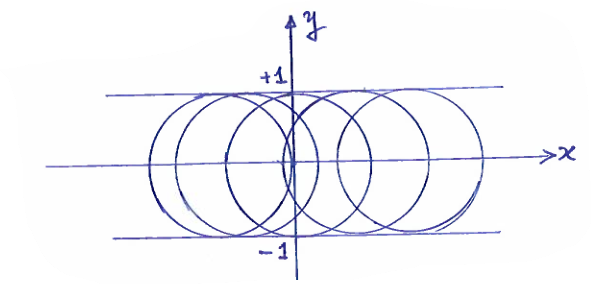
\includegraphics[height=0.5\textheight, width=0.5\textwidth, keepaspectratio]{./Images/normal_envelop_05.png}
	\end{center}
\end{figure}
Nessa situação, os círculos ``se acumulam'' ao longo das retas \(y=-1\) e \(y=+1\), que são tangentes a \textit{todos} os círculos da família. De certo modo, elas podem ser consideradas como o limite do pontos de interseção dos círculos; estas retas \(y=\pm 1\) são o \textbf{envelope da família dos círculos.}

Tentaremos replicar essa ideia para uma curva \(\alpha \) que não seja um círculo: tomemos \(\alpha :I\rightarrow \mathbb{R}^{2}\) uma curva parametrizada p.c.a. Encontrar o envelope das retas normais a ela significa achar o lugar onde as retas normais se acumulam, seguindo a ideia vista acima.
Sabemos que um ponto \(X\in \mathbb{R}^{2}\) pertence à reta normal à curva \(\alpha \) em s se, e somente se,
\[
	\langle X-\alpha (s), t(s) \rangle=0.
\]
Com isso, está motivada a definição
\begin{def*}
	Suponha que \(\alpha\) é parametrizada p.c.a e considere a família de funções
	\begin{align*}
		F: & I\times \mathbb{R}^{2}\rightarrow\mathbb{R}^{2}                        \\
		   & (s, x)\longmapsto F(s, x)\coloneqq \langle X-\alpha (s), t(s) \rangle.
	\end{align*}
	O \textbf{envelope (discriminante)} da família F é o conjunto
	\[
		\mathcal{D}=\biggl\{ x\in \mathbb{R}^{2}:\; \exists s\in I,\; F(s, x) = \frac{\partial^{}F}{\partial s^{}}(s, x)=0\biggr\}. \; \square
	\]
\end{def*}
\begin{figure}[H]
	\begin{center}
		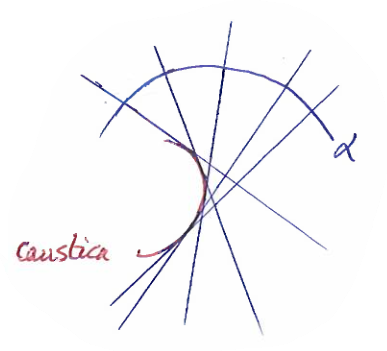
\includegraphics[height=0.5\textheight, width=0.5\textwidth, keepaspectratio]{./Images/circle_envelop_05.png}
	\end{center}
	\caption{se pensarmos na curva como uma fonte de luz, o envelope vai ser os pontos mais iluminados do plano, e por isso ele também é conhecido como ``caustica''!}
\end{figure}

De fato, a definição dada se justifica, pois se considerarmos \(\gamma (s)\) como uma curva tangente a todos os membros da família \(F(s, x)=0\), isso constitui exatamente todas as curvas com equação
\[
	F_{s}(x)\coloneqq F(s, x)=0;
\]
assim, para todo s em I, \(F(s, \gamma (s))=0\), e temos
\[
	\frac{\partial^{}F}{\partial s^{}}(s, \gamma (s))+\biggl\langle \nabla F_{s}(s, \gamma (s)), \gamma'(s) \biggr\rangle=0.
\]
Daí, a curva \(\gamma \) é tangente aos membros da família F se, e somente se,
\[
	\biggl\langle \nabla F_{s}(s, \gamma (s)), \gamma'(s) \biggr\rangle=0 \Longleftrightarrow \frac{\partial^{}F}{\partial s^{}}(s, \gamma (s))=0.
\]
Disto, concluímos que \(\gamma \) é o envelope das curvas \(F_{s}(x)=0\) se, e somente se, seu traço faz parte do envelope \(\gamma (I)\subseteq \mathcal{D}\).

\begin{prop*}
	O envelope da família das retas normais a uma curva \(\alpha \) é a evoluta da curva.
\end{prop*}
\begin{proof*}
	Queremos achar os pontos x em \(\mathbb{R}^{2}\) tais que, para algum s em I,
	\[
		F(s, x)=\frac{\partial^{}F}{\partial s^{}}(s, x)=0.
	\]
	Equivalentemente,
	\begin{align*}
		F(s, x)= \langle x-\alpha (s), t(s) \rangle =0 & \Longleftrightarrow x-\alpha (s)=\lambda n(s)    \\
		                                               & \Longleftrightarrow x = \alpha (s)+\lambda n(s).
	\end{align*}
	Por outro lado,
	\[
		\frac{\partial^{}F}{\partial s^{}}(s, x)=-\langle t(s), t(s) \rangle + \langle x-\alpha (s), \kappa '(s)n(s) \rangle.
	\]

	Logo,
	\[
		F(s, x)=\frac{\partial^{}F}{\partial s^{}}(s, x)=0 \Longleftrightarrow x = \alpha (s)+\lambda n(s)\quad\&\quad \lambda \kappa (s)-1=0.
	\]
	Portanto,
	\[
		x = \alpha (s)+\frac{1}{\kappa (s)}n(s) = e(s). \text{ \qedsymbol}
	\]
\end{proof*}

\subsection{Sobre Propriedades Globais}
Agora que temos alguns itens em nossa ontologia de geometria diferencial, podemos mencionar alguns dos problemas da área, e fornecer o enunciado do teorema dos quatro vértices, mesmo que sua demonstração tenha ficado como enunciado.
Sem mais delongas,
\hypertarget{four_vertices}{
	\begin{theorem*}[Teorema dos Quatro Vértices]
		Uma curva plana, regular, simples e fechada contém pelo menos dois pontos distintos de máximo local e dois pontos distintos de mínimo local da curvatura \(\kappa \) da curva.
	\end{theorem*}
}
\begin{proof*}
	Seminário. \qedsymbol
\end{proof*}

Apesar de ser uma área bem antiga, anida existem muitas questões a serem ponderadas na geometria diferencial. Servindo de motivação, vamos ver algumas delas:
\begin{example}[Problemas sobre Curvas Planas]
	\begin{itemize}
		\item[1.)] \textbf{\underline{Conjectura}:} Seja \(\alpha (u)=(u, P_{n}(u)\) o gráfico de um polinômio de grau n. Então, a curva \(\alpha \) possui no máximo (n-1) vértices.
		\item[2.)] \textbf{\underline{Conjectura}:} Como podemos definir a curvatura de uma curva holomórfica em \(\mathbb{C}^{2}\)?
		\item[3.)] \textbf{\underline{Conjectura}:} Seja \(\alpha_{0} (u)=(u^{2}, u^{3}\), com \(u\in (-\varepsilon , \varepsilon )\), uma curva com singularidade do tipo cúspide. Podemos deformar a curva \(\alpha_{0}\) variando t perto de zero n família de curvas \(\alpha_{t}(u)=(u^{2}, u^{3}+tu)\), exibindo seus pontos de inflexão e seus vértices;
		      neste contexto, os seguintes problemas são de interesse: dada uma curva singular, parametrizada por \(\alpha :(-\varepsilon , \varepsilon )\rightarrow \mathbb{R}^{2}\), ou dada pela equação \(f(x, y)=0,\; f:(0,0)\in U\subseteq \mathbb{R}^{2}\rightarrow \mathbb{R}\),
		\item[3.i)] Quantos pontos de inflexão e vértices estão ``armazenados'' na singularidade?
		\item[3.ii)] Existem modelos de deformações da curva que exibem a maneira como os pontos de inflexão e vértices aparecem nas deformações da curva, conhecidas como \textbf{deformações geométricas}?
		      \begin{figure}[H]
			      \begin{center}
				      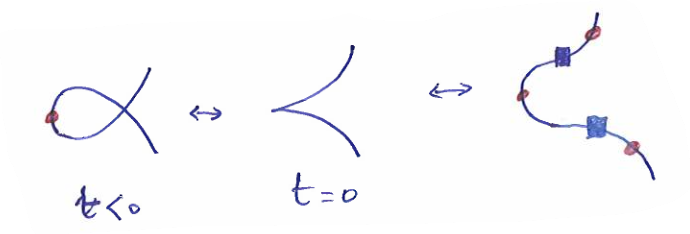
\includegraphics[height=0.7\textheight, width=0.7\textwidth, keepaspectratio]{./Images/cuspid_05.png}
			      \end{center}
			      \caption{os {\color{Red2}vértices} e {\color{Blue3}pontos de inflexão} que surgem deformando a singularidade aparecem indicados na figura.}
		      \end{figure}
	\end{itemize}
\end{example}
\end{document}
